% F1: ParBench System Architecture Diagram
% Standalone TikZ document — compile with: pdflatex f1_system_architecture.tex
% SC26 outfit-derived palette
\documentclass[border=8pt]{standalone}
\usepackage{tikz}
\usetikzlibrary{arrows.meta, positioning, fit, calc, shapes.geometric}

% SC26 palette colors
\definecolor{teal}{HTML}{2E8E9E}
\definecolor{tealtint}{HTML}{D8F0F4}
\definecolor{rosepink}{HTML}{C8607A}
\definecolor{rosetint}{HTML}{F8E0E5}
\definecolor{saffron}{HTML}{D48A35}
\definecolor{saffrontint}{HTML}{FBF0DD}
\definecolor{gold}{HTML}{E6A84D}
\definecolor{goldtint}{HTML}{FDF5E3}
\definecolor{charcoal}{HTML}{2D3436}
\definecolor{slate}{HTML}{636E72}
\definecolor{linen}{HTML}{F5F0EB}

\begin{document}
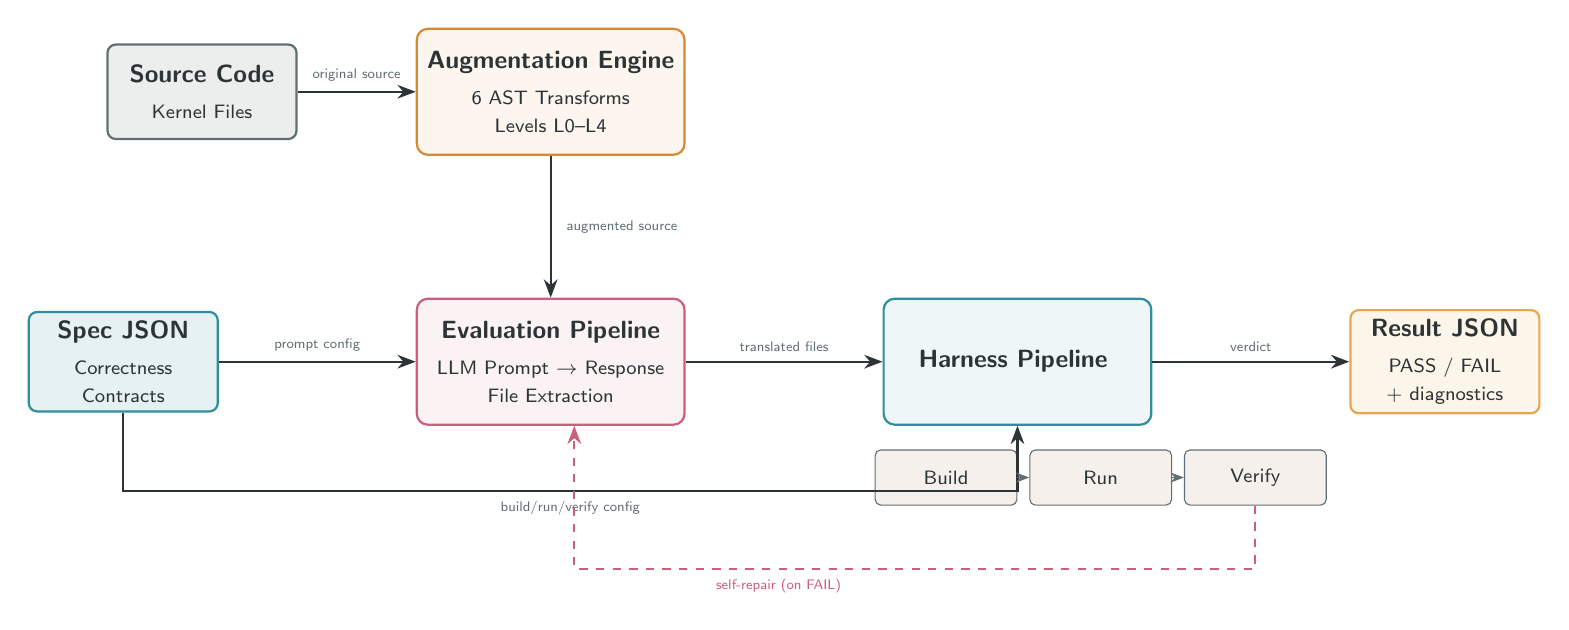
\begin{tikzpicture}[
    >=Stealth,
    node distance=1.6cm and 2.2cm,
    box/.style={
        draw=#1, fill=#1!8, thick, rounded corners=4pt,
        minimum width=3.4cm, minimum height=1.6cm,
        font=\sffamily\small, align=center, text=charcoal
    },
    smallbox/.style={
        draw=slate, fill=linen, rounded corners=2pt,
        minimum width=1.8cm, minimum height=0.7cm,
        font=\sffamily\scriptsize, align=center, text=charcoal
    },
    iobox/.style={
        draw=#1, fill=#1!12, thick, rounded corners=3pt,
        minimum width=2.4cm, minimum height=1.2cm,
        font=\sffamily\small, align=center, text=charcoal
    },
    arrow/.style={->, thick, color=charcoal},
    darrow/.style={->, thick, dashed, color=rosepink},
    label/.style={font=\sffamily\tiny, text=slate}
]

% === Main flow (left to right) ===

% Spec JSON (input)
\node[iobox=teal] (spec) {
    \textbf{Spec JSON}\\[2pt]
    {\scriptsize Correctness}\\[-1pt]
    {\scriptsize Contracts}
};

% Evaluation Pipeline (center)
\node[box=rosepink, right=2.5cm of spec] (eval) {
    \textbf{Evaluation Pipeline}\\[2pt]
    {\scriptsize LLM Prompt $\to$ Response}\\[-1pt]
    {\scriptsize File Extraction}
};

% Harness Pipeline (right)
\node[box=teal, right=2.5cm of eval] (harness) {
    \textbf{Harness Pipeline}
};

% Harness sub-stages
\node[smallbox, below=0.3cm of harness.south west, anchor=north west, xshift=-0.1cm] (build) {Build};
\node[smallbox, right=0.15cm of build] (run) {Run};
\node[smallbox, right=0.15cm of run] (verify) {Verify};

% Result JSON (output)
\node[iobox=gold, right=2.5cm of harness] (result) {
    \textbf{Result JSON}\\[2pt]
    {\scriptsize PASS / FAIL}\\[-1pt]
    {\scriptsize + diagnostics}
};

% Augmentation Engine (above, branching into eval)
\node[box=saffron, above=1.8cm of eval] (augment) {
    \textbf{Augmentation Engine}\\[2pt]
    {\scriptsize 6 AST Transforms}\\[-1pt]
    {\scriptsize Levels L0--L4}
};

% Source Code (above-left, feeds into augmentation)
\node[iobox=slate, left=1.5cm of augment] (source) {
    \textbf{Source Code}\\[2pt]
    {\scriptsize Kernel Files}
};

% === Arrows ===

% Source -> Augmentation
\draw[arrow] (source) -- (augment)
    node[label, midway, above] {original source};

% Augmentation -> Evaluation
\draw[arrow] (augment) -- (eval)
    node[label, midway, right, xshift=2pt] {augmented source};

% Spec -> Evaluation (prompt generation)
\draw[arrow] (spec) -- (eval)
    node[label, midway, above] {prompt config};

% Spec -> Harness (verification config)
\draw[arrow] (spec.south) -- ++(0, -1.0) -| (harness.south)
    node[label, pos=0.25, below] {build/run/verify config};

% Evaluation -> Harness (translated files)
\draw[arrow] (eval) -- (harness)
    node[label, midway, above] {translated files};

% Harness -> Result
\draw[arrow] (harness) -- (result)
    node[label, midway, above] {verdict};

% Build -> Run -> Verify internal arrows
\draw[arrow, thin, color=slate] (build) -- (run);
\draw[arrow, thin, color=slate] (run) -- (verify);

% Self-repair feedback loop (Verify -> Evaluation)
\draw[darrow]
    (verify.south) -- ++(0, -0.8) -| ($(eval.south) + (0.3, 0)$)
    node[label, pos=0.35, below, text=rosepink] {self-repair (on FAIL)};

\end{tikzpicture}
\end{document}
